%!TEX root = main.tex
\chapter{Problem Elaboration}
\label{chap:problemelaboration}
\label{problemelaboration}
In this chapter we will elaborate on our problem by defining our task and presenting our high level requirements. We will also introduce GitHub as the choice of version-control system for our implementation.
On the basis of theory, background and related work we will also also present our two main scenarios and the context of these. 

\section{Problem Overview}
\label{problemdefinition}

To answer our research questions we will develop a web-tool aimed at software development teams adopting an agile process model. Most agile process models adopt reflection sessions \citep{retrospectivedzone}, and helping users prepare for these sessions in order to gain the best possible learning outcome is one of the main issues our tool try to address. Collecting experience related data throughout a working day, allows users to revisit recent(fresh) experiences and trigger reflection upon these experiences. By capturing these daily reflections and storing them for later use allow users to go back to these experiences and recollect the lessons learned. Sharing these notes with the rest of the team allows the team to collaboratively prepare for the retrospective sessions that take place in agile process models. Reviewing these daily reflection notes individually by the user and/or by the team, further helps identify trending issues spanning the iteration and even the whole project over time. The team can also use the shared notes to compare experiences and trigger discussion and reflection upon these. 

Most of these teams use some sort of a version control system with project artifact's, like programming code, text documents etc. We have chosen to focus on GitHub(See section \ref{githubchapter}), but the tool could be adapted to work with any version tracker that allows for data collection. \\
Figure \ref{overalltoolprocess} shows the overall process of our application, how user's interact with GitHub and the PeacefulBanana application. 

\begin{figure}[H]
\centering
	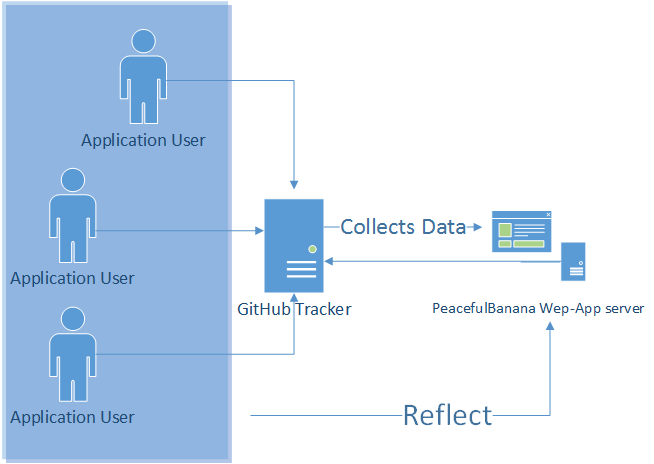
\includegraphics[width=\textwidth]{overalltoolprocess}
\caption{Overall application process}
\label{overalltoolprocess}
\end{figure}

The tool will collect relevant data from the project repository on GitHub without any action needed from the user to do so. The tool will then \emph{scaffold}, that is present the collected data in a structured frame in order to allow users to revisit and reflect upon agile project experiences, and also share these reflection notes.

The experiences will be presented in several different ways like activity-graphs, mood-graphs and tag clouds. These will act as reflection triggers and help the users to reflect on their work. These experiences will be collected and made available for the users and/or the team later. The tool will be designed with reflection in mind, and scenarios was created to demonstrate the most important functionality regarding enhancing reflection in software development teams. Although we evaluate the application in the context of demonstrative scenarios, we see the possibility of the application being used outside of the context provided by scenarios. Users can at any time look into a repository, a milestone or a single issue and the tool will provide data that is useful for recollecting experiences and providing a basis for reflection upon these. 

We have worked out two main scenarios, which can be seen in Section \ref{sec:scenarios}. Evaluation of the application will be conducted in the context of these in order to gain feedback on how the application may answer our research questions. Evaluation will be a usability test, an expert review and a focus group. 

\section{Github}
\label{githubchapter}
This section will introduce GitHub, the features GitHub provides and the rationale behind choosing GitHub as the VCS for our tool implementation. 
GitHub is a web-based hosting service for software development projects that use the Git revision control system\citep{git,github}. GitHub offers both paid plans for private repositories, and free accounts for open source projects.

GitHub provides users with integrated issue tracking, code review, project wiki, useful statistics and more. 
Motivational points for choosing GitHub as the revision control system to integrate with are several. Some technical aspects are that GitHub provides developers with a simple to use API\citep{githubapi}, with libraries for integration with most of the commonly used programming languages, like Java\citep{jgit}.

In addition to the technical aspects, GitHub is the most used revision control system ,as of January 2013 GitHub announced it had passed the 3 million users mark and now hosting more than 5 million repositories and is a tool many in our evaluation group already use in their development projects\citep{githubnumbers}.

\subsection{Authentication}
The application features an authentication with GitHUb, through the use of OAUTH2 tokens. When the user first uses the tool, he will be asked to authenticate with GitHub's authentication page, asking the user to log in and authorize the PeacefulBanana tool. When this is done the tool receives a token it can use on behalf of the user to retrieve data from GitHub. The token itself is not stored, but retrieved in the background when required and bound to the users HTTP-session which expires when the user closes the browser window. This is done for safety reasons cause it would be devastating if these tokes got in the hands of the wrong people, they could for example delete the entire repository.

For gathering data from GitHub, this data is transfered as JSON(JavaScript Object Notation), a lightweight data interchange language. You can see all the possible data-types gathered from the GitHub API.
\subsection{Repositories}
GitHub is a repository hosting service for software development projects. A repository contains all the project files, may it be code, images, and other documentation. This means that all content in a project is connected to this repository. In addition to documentation and file content, GitHub provides integrated issue tracking, which is connected to this repository and could also be connected to one or several milestones. 
\subsection{Commits}
Say some of your project files have been changed, for example some code snippet in a Java file. The way to save these changes to your local branch is by commits. A commit can consist of code line additions, deletions, files added, changed or removed. When you are ready to save the changes, you commit them in a command line together with a commit message which is a short text describing the changes you have done. \\
When a user is ready to push one or more local commits to the project repository, it can be done via the command git push in the command line. It is now the HEAD revision and the new code and commits can be seen on the GitHub page.
\subsection{Milestones and Issues}
\begin{quote}
\em GitHub Issues can be assigned to a user to make it easy to know who's working on what, or which issues you need to tackle next.
\end{quote}
Every GitHub repository has an issue tracker, that allows users to track bugs and focus on features. Milestones and issues help manage large projects, where issues especially makes for a great TODO list, similar to a product backlog. Only {\bf collaborators} can create and view issues on private repositories. On public repositories anyone can create and view issues. 
\begin{itemize}
\item GitHub issues can be assigned to a user, which makes it easy to know who's working on what, or which issues should be handled next. Milestones are a good way of helping team members to work towards a goal. A team can set a due date, name a milestone and then start assigning issues to that milestone. An example of a Milestone could be a due date of a project demo or delivery. Any number of issues can then be assigned to this milestone, and thus be connected to it. 
\item Issues know all about commits. GitHub enables referencing and closing issues with Commit Messages. By using a few simple keywords you can close an issue right from a commit message, or just leave a note on the issue.The syntax to do this is as follows: To close issue \#35 , a commit message containing 'closes \#35' , will close issue number 35 when pushed to GitHub. Other keywords are: close, closes, closed, fixes, fixed. 

To leave a note on issues can be done by simply mentioning the issue number without any keywords in a commit message. F.ex "This commit references \#35". Anyone with write access to a repository may close an issue or leave a note.
\end{itemize}

\section{Reflection and technology}
% Why is reflecting important and what are the challenges.
The world wide web and modern technologies provides easy access to enormous amounts of information. This means that in order to learn, learners must be able to make sense of the information collected.  
In order to achieve this and make conscious decisions of how to use information, learners need to reflect on the information they collect. Reflection upon the process of solving problems is necessary to achieve a good result and to improve the ability to learn from experiences. When supporting learning with technology, this technology should promote these aspects within learning\citep{Lin1999}

The main goal is to provide technology that enables efficient information retrieval, and to provide scaffolds or frames that support reflective thinking and problem solving. In our task this means utilizing collaborative learning experiences. 

\subsection{Agile Retrospective}
The agile retrospective is held at the end of an iteration in order to learn from the iteration and not repeat mistakes. A model of how a retrospective can be done is shown in \citep{Derby2006}. The purpose is to learn what works and what does not work, and make the adjustments necessary for the next iteration. This way the team makes sure that every iteration introduces some improvements in the team's process. There are two fundamental questions the retrospective is intended to answer:
\begin{itemize}
\item What went well during the last iteration that we continue doing?
\item What could we do differently in order to improve?
\end{itemize}
Figure \ref{fig:itcyclemodel} is a model of where the retrospective fits in the agile iteration cycle, and the table in Figure \ref{fig:retrospectivetable} shows the process in more details, from beginning to end.\citep{Derby2006}:
\begin{figure}[!htpb]
\centering
	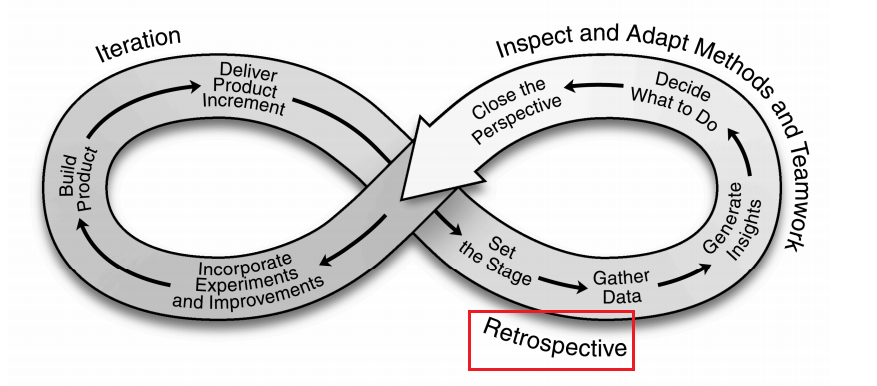
\includegraphics[width=\textwidth, keepaspectratio=true]{iterationcyclemodel}
\caption{Retrospectives in the agile iteration cycle \citep{Derby2006}}
\label{fig:itcyclemodel}
\end{figure}
\begin{figure}[!htpb]
\centering
	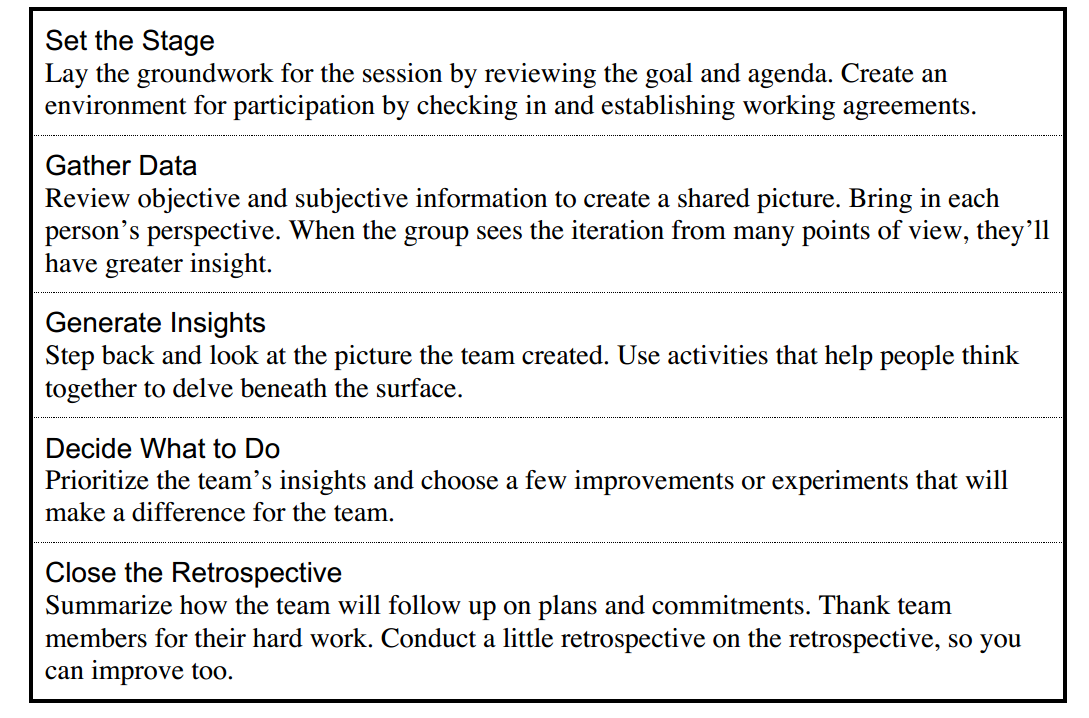
\includegraphics[width=\textwidth, keepaspectratio=true]{retrospectivetable}
\caption{Agile retrospectives - from beginning to end \citep{Derby2006}}
\label{fig:retrospectivetable}
\end{figure}
\\
The agile manifesto, also introduces some key practices guidelines aimed towards retrospectives in Scrum teams\citep{agilemanifesto}:
\begin{enumerate}
\item Meeting Customer satisfaction: The Retrospective can be used to reflect on how well the Scrum Team is addressing the customer satisfaction.
\item Welcoming Changing requirements: The Retrospective is a good venue to assess if the Product Backlog is evolving and therefore the Scrum Team and Product Owner are flexible enough.
\item Delivering working software regularly: The result and feedback received during the iteration Review can be analyzed during the iteration Retrospective to assess this element.
\item Working together: Reflection on how well the business and technical people are working together is a good activity to ensure that the environment fosters communication between those 2 groups.
\item Giving support and trust: The Scrum Team can self-assess and also assess if management has provided an appropriate infrastructure.
\item Fostering face-to-face conversation: The quality and frequency of the face-to-face conversation is a point that can be analyzed during a iteration Review.
\item Delivering working software: Assessing the quality of the key deliverable to date is of essential value.
\item Having a sustainable structure: Signs that could conclude that the project is not sustainable must be discussed.
\item Technical excellence: As for point 6, quality is a non-negotiable aspect of Scrum and should be reviewed during the retrospective.
\item Keeping the system simple: Signs of an unnecessary complex system should be discussed.
\item Working in self-organizing team: Evidences that the Scrum Team is hindered because not self-managed should be analyzed.
\item Regular reflection: The Scrum Retrospective being such activity, this will always be true!
\end{enumerate}

\section{Scenarios}
\label{sec:scenarios}

Based on related work, we have developed two scenarios to show what we want our tool to support in terms of collaborative reflection and learning. These two scenarios will provide a basis for the requirement elaboration and design choices in development of the tool. 
\\
At the Norwegian University of Science and Technology, NTNU, a group of students are taking the course IT2901 - Informatics Project II\footnotemark.
In the course, the focus is not only on the project itself, but also on the process the group steps through in order to reach their goal, including group roles, distribution of work etc. At the end of the course, students have to present a product report, with their project results, and a process report, with their project process results and experiences. In addition to this, groups participate in a retrospective workshop at the end of the course. In these three scenarios, our users are students and part of a group in the course , with age ranging from 22 and up to 28 years old.
\\
The group is going to work on a customer-driven project, using an agile methodology like scrum. The group will be using GitHub as a version-control system. During the project work the team will use GitHub to collect information. The PeacefulBanana tool can then be used to gather this information and present it in a scaffolded way mainly to be used in reflection sessions. Users can though, at any time go into the application and gather relevant data if they want to. This data will help the group to see trending issues and problems they have come upon in the process. Each member of the group will register as a user on the PeacefulBanana tool. The users will then be connected together as a group. 
\\
The two scenarios described in the next sections provides examples of how we envision the usage of the PeacefulBanana tool in three different settings. First as a individual tool on a daily basis, then as part of a team collaborative reflection session.
These two scenarios were developed early in the development process. The first scenario features using the tool at the end of each working day as inspired by [ref to the 5 minute daily reflection session]. The second scenario where in the end of each iteration there is a retrospective reflection session. 
\\

\footnotetext{Informatics Project II is a course where students from the Informatics education program is put together in groups working on different software development projects. Key objectives of this course are gaining practical experience in GROUP-ORIENTED software engineering for a customer, covering the whole life-cycle of a software project - \url{http://www.ntnu.edu/studies/courses/IT2901}}

\subsection{Scenario 1 - Individual use on a daily basis}
\label{scenario1}
In this scenario, our students will be using the tool on a daily basis at the end of each working day.

When the students enter the web-application, they will get a notification with a prompt to do the daily status update.

\begin{figure}[h!]
\label{newnotification}
\centering
	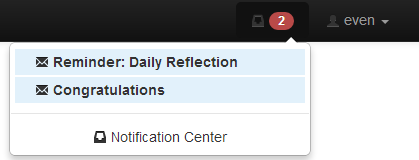
\includegraphics[width=\textwidth]{newnotification}
\caption{The user has clicked the notification icon and can see his new notifications}
\end{figure}

  When clicking the notification, the student is presented with a summary of their individual activity in the last 24 hours.
  This summary compares the commit activity of the user with the team's, and also presents a tag cloud representing the trending issues of the last day. The user is then prompted to input todays mood, their top two contributions \emph{"What did I do good?"} , and their top 2 points to improve on \emph{"What could I do better?"}. Finally the user can submit the form and choose to share these experiences with the team for collaborative use. The daily reflection notes are saved and can be reviewed at any time, and also shared any time by the user. The idea is that the tool will be used to revisit todays experiences with collected information presented in a way that triggers reflection upon these experiences. Information is collected and inspire new experiences. After working on a project that day, students "step back" to reflect on what happened during the day, and on the experiences they encountered. The tool provides scaffolded data to further trigger this reflection process. This process consist of returning to the experiences of that day, re-visit the experiences and attend to the feelings, like inputing todays mood. This reflection will help users to derive their top two improvements and contributions of the day\citep{Krogstie2011}. The tool thus captures the experiences and reflections made by the user and allows for re-visiting of these at a later date by storing them in the system. 

\subsection{Scenario 2 - Team use after each iteration}
\label{scenario2}
In this scenario, students will be using the tool as part of the agile methodology reflection sessions. Students will individually be able to use the tool as a preparation for these sessions, while the team can use the tool collaboratively towards the session as well.
In this scenario, the students will be using the tool as a part of the agile scrum methodology two-week reflection sessions. Students will in this scenario use the tool to indicate how the project has been progressing over the last iteration, tightly coupled with one or several milestones. The students will generate tag clouds based on the trending issues in the relevant milestones, activity graphs and mood trajectories. Also if the users have chosen to share any of the individual reflection notes from scenario 1, these will be visible and can be used to draw conclusions from the previous iteration, and make comparisons. The tool will enable a group to see the whole iteration more clearly, but also be able to dive into certain issues or milestones that showed to be of particular interest, and thus create a discussion around the experiences made by the team members.  